\Chapter{Node Package Manager (npm)}

\Section{Bevezetés}

Ennek a fejezetnek a célja, hogy az npm technológia a szakdolgozat és a készítendő program szempontjából releváns területei feltárásra és bemutatásra kerüljenek.

Az npm a világ legnagyobb szoftver nyilvántartása. A fejlesztők segítségével megoszthatják az általuk fejleszett csomagokat, használhatják a mások által írtakat, illetve ezen funkcionalitást gyakran kiaknázzák nagyobb szervezetek a belső fejlesztésekhez.

A csomagkezelő három, jól megkülönböztethető részből épül fel:
\begin{itemize}
	\item A weboldal
	\begin{itemize}
		\item Alapvetően itt lehet megkeresni különböző csomagokat, lehetséges saját profil létrehozása, illetve az npm használatának aspektusait is be lehet állítani.
	\end{itemize}
	\item A CLI (Command Line Interface, azaz parancssoros felület)
	\item Az npm registry (Adatbázis)
\end{itemize}

\begin{flushright}
\cite{npm-about}
\end{flushright}

\Section{npm Csomagok}

Egy csomag egy \emph{package.json} fájl által megadott fájl vagy könyvtár. A csomagnak így mindenképpen tartalmaznia kell a korábban említett \emph{package.json} fájlt, mivel enélkül nem lehetséges az npm nyilvántartásba feltölteni.\\

Általánosságban egy csomag legalább az alábbiakat tartalmazza: 

\begin{itemize}
	\item Belépési pont (Pl. \emph{index.js})
	\item \emph{package.json}
	\item README (Információk a csomagról)
	\item CHANGELOG (A csomagverziók szerinti változtatások nyilvántartása)
	\item LICENSE (A csomag licensze)
\end{itemize}

A csomagoknak az \underline{alábbiakat nem szabad / nem célszerű} tartalmaznia:

\begin{itemize}
	\item Nagy méretű fájlok
	\item Érzékeny információk
	\item Csak a fejlesztéshez szükséges eszközök
	\item Eszköz konfigurációs fájlokat (Pl. \emph{babel.config.json})
	\item Log fájlokat
\end{itemize}

\begin{flushright}
	\cite{npm-packages}
\end{flushright}

	\subsection{\emph{package.json}}
	
	A \emph{package.json} fájl a legfontosabb a csomagok pubkilálása szempontjából. Amennyiben egy fejlesztő közzé szeretné tenni egyik csomagját, abban az a minimális követelemény a fájllal szemben, hogy tartalmazza a kötelező mezőket.
	
	Nagyon sok mezőt tartalmazhat, akár felhasználó által definiáltakat is, kulcsfontosságú a készítendő program szempontjából is, mivel tartalmazza a csomag függőségeit, hogy ezek mely verziói elfogadottak.
	
	A \emph{package.json} az alábbi mezőket tartalmazhatja (a teljesség igénye nélkül):
	
	\begin{itemize}
		\item \textbf{Kötelező:}
		\begin{itemize}
			\item \texttt{"name"} (Csomagnév)
			\begin{itemize}
				\item Ez a mező tartalmazza a csomag nevét, melynek az npm elnevezési konvenciót kell követnie. (Bővebben: \hyperlink{subsection.2.2.2}{\underline{Csomag Elnevezési Konvenciók}})
			\end{itemize}
			\item \texttt{"version"} (Csomag verzió)
			\begin{itemize}
				\item Követnie kell az npm szemantikus verziózási szabályait. (Bővebben: \hyperlink{subsection.2.2.3}{\underline{Szemantikus Verziózási Szabályok}}) 
				\item x.x.x formában kell megadni
			\end{itemize}
		\end{itemize}
		\item \textbf{Opcionális:}
		\begin{itemize}
			\item \texttt{"description"} (A csomag keresését könnyítő leírás)	
			\item \texttt{"scripts"} (Futtatható npm scriptek)
			\item \texttt{"repository"} (A csomag GitHub-on vagy egyéb verziókezelő rendszerben nyilvántartott repositoryja)
			\item \texttt{"keywords"} (A csomag keresését könnyítő kulcsszavak)
			\item \texttt{"license"} (Licensz a csomag felhasználásának szabályairól)
			\item \texttt{"author"} (Csomag tulajdonos, szerző)
			\item \texttt{"contributors"} (Közreműködők)
			\item \texttt{"bugs"} (Ismert hibák)
			\item \texttt{"homepage"} (A csomagot ismertető weboldal)
			\item \texttt{"files"} (Megadható, hogy a csomag csak megadott fájlokat  tartalmazzon)
			
			\clearpage
			
			\item \texttt{"dependencies"} (A csomag használatához szükséges függőségek)
			\begin{itemize}
				\item Nem kötelező, azonban, ha van függőség, a csomag telepítése során csak az itt megjelölt csomagokat fogja telepíteni a csomagon kívül, így ha itt nincs megjelölve egy csomag melynek funkcionalitására épül az aktuális projekt, könnyen lehet, hogy futás közben hibába fog ütközni.
			\end{itemize}
			\item \texttt{"devDependencies"} (A csomag fejlesztéséhez, fordításához szükséges függőségek)
			\item \texttt{"optionalDependencies"} (Opcionális függőségek)
		\end{itemize}
		\item \textbf{Továbbiak:}
		\begin{itemize}
			\item A lehetőségek tárháza nagy, akár saját adatokkal is bővíthetjük a \emph{package.json} fájlt 
		\end{itemize}
	\end{itemize}

	\begin{flushright}
		\cite{npm-package.json}
	\end{flushright}
	
	\subsection{Csomag Elnevezési Konvenciók}
	
	Az npm csomagok elnevezésénél első lépésként meg szükséges határozni, hogy úgynevezett "scoped" vagy "unscoped" csomagról beszélünk.
	
	A "scope"-ot vagy "hatáskör"-t akkor célszerű alkalmazni, ha az összetartozó csomagokat szeretnénk egy csoportba rendezni. A csomagnév elé írt '@' karakterrel lehet jelezni, hogy "scoped" csomagról van szó.
	
	\begin{cpp}
@scope/packagename
	\end{cpp}

	Ilyenkor természetesen a "scope" lehet ugyanaz több csomag esetén is, ezzel jelezve, hogy összetartozó csomagokról van szó.
	Erre példa lehet az Angular keretrendszer esete, ahol a fejlesztői csomagok az @angular-devkit "scope"-ot használják.
	
	\begin{cpp}
@angular-devkit/architect
@angular-devkit/core
@angular-devkit/schematics
	\end{cpp}

	Mind a "scoped" és "unscoped" csomagoknak azonban be kell tartaniuk az alapvető \textbf{elnevezési konvenciókat:}
	
	\begin{itemize}
		\item A csomagnévnek egyedinek kell lennie
		\item Az elnevezés utaljon a funkcionalitásra
		\item Ne ütközzön az npm irányelveibe, illetve ne legyen védjegy alatt az elnevezés
		\item Ne tartalmazzon szóközöket
		\item Tartalmazhat alsóvonást, illetve kötőjelet
		\item "unscoped" csomagok esetében:
		\begin{itemize}
			\item Ne legyen az elnevezés más tulajdonában
			\item Ne legyen hasonló más csomagnévhez
			\item Ne zavarjon össze másokat a tulajdonos személyével kapcsolatban
		\end{itemize}
	\end{itemize}

	\begin{flushright}
		\cite{npm-scope} \cite{npm-naming}
	\end{flushright}

	\subsection{Szemantikus Verziózási Szabályok}
	
	Ahhoz, hogy a JavaScript ökoszisztéma egészséges, megbízható és biztonságos legyen, minden jelentős változtatás után javasolt az csomag egy újabb verzióját publikálni, amelyet az adott \emph{package.json} fájlban szükséges feltüntetni. A csomag verzióinak megadásánál fontos követni a szemantikus verziózási szabályokat, mivel így más fejlesztőknek, akiknek projektjük az aktuális csomagtól függ, egyszerűbb lesz alkalmazkodnia az időközi változásokhoz.
	
	A csomagok verziójának megadásánál az \textbf{x.x.x} forma az elfogadott.
	
	A csomagok fejlődésénél alapvetően 4 különböző szakaszt különböztetünk meg, ezeknek szabályai:
	
	\begin{table}[h]
		\centering
		\caption{Csomagok fejlődésének szakaszai:}
		\label{tab:package-lifecycle}
		\begin{tabular}{|c|c|c|}
			\hline
			\textbf{Szakasz} & \textbf{Szabály} & \textbf{Példa} \\
			\hline
			Új csomag & Első verzió: 1.0.0 & 1.0.0 \\
			\hline
			„Patch” kiadás & A 3. számjegyet növeljük & 1.0.1 \\
			\hline
			Kisebb (Minor) kiadás & A 2. számjegyet növeljük & 1.1.0 \\
			\hline
			Jelentős (Major) kiadás & Az 1. számjegyet növeljük & 2.0.0 \\
			\hline
		\end{tabular}
	\end{table}

	Minden új verzió esetén a csomag publikálásakor egy újabb bejegyzés jön létre az npm Registry-ben, illetve az új verziószám hozzáadódik a csomag bejegyzés verzióihoz.
	
	A \emph{package.json} fájlban, így a Registry bejegyzésben is szereplő függőségi verziókövetelményben megadhatóak mely verziót vagy verziókat fogadja el az adott csomagból. Ezeknek megadására több lehetőség is létezik, azonban szigorú szintaktikai szabályokhoz van kötve:
	\begin{table}[h]
		\centering
		\caption{Verziózás szintaktikai szabályai:}
		\label{tab:sem-ver-pt1}
	\begin{tabularx}{\textwidth} { 
			| >{\centering\arraybackslash}X 
			| >{\centering\arraybackslash}X 
			| >{\centering\arraybackslash}X | }
		\hline
		\textbf{Szabály} & \textbf{Szintaktika} & \textbf{Példa} \\
		\hline
		Minden verzió, amely esetén az első nem 0 számjegy nem nő & \textsuperscript{$\wedge$}x.x.x & \textsuperscript{$\wedge$}0.2.0 esetén:\newline $\big[$0.2.x; 0.3.0$\big[$ \\
		\hline
		Minden verzió, amely nagyobb a megadottnál ugyanabban a Minor tartományban & $\sim$x.x.x & $\sim$2.2.0 esetén:\newline $\big[$2.2.x; 2.3.0$\big[$  \\
		\hline
		Stabil verziók tartományának megadása & \underline{Összehasonlítások:} <, >, =, <=, >= \underline{Inkluzív tartomány:} - (A kötőjel mindkét oldalán 1 szóköz karakternek kell szerepelnie!) & >3.1 esetén: \newline Minden 3.1-nél nagyobb verzió 2.0.0 – 2.3.0 esetén: $\big[$2.0.x; 2.3.x$\big]$ \\
		\hline
		Kiadás előtti (alfa, béta) verzió & x.x.x-rc.x (Csak pontos verziót lehet megadni) & 1.0.0-rc.1 \\
		\hline 
	\end{tabularx}
	\end{table}

	\clearpage

	\begin{table}[h]
		\caption{Verziózás szintaktikai szabályai (folytatás):}
		\label{tab:sem-ver-pt2}
		\begin{tabularx}{\textwidth} { 
				| >{\centering\arraybackslash}X 
				| >{\centering\arraybackslash}X 
				| >{\centering\arraybackslash}X | }
			\hline
			\textbf{Szabály} & \textbf{Szintaktika} & \textbf{Példa} \\
			\hline 
			Kiadás előtti (alfa, béta) verziók tartományának megadása & \underline{Összehasonlítások:} <, >, =, <=, >= \underline{Inkluzív tartomány:} - (Csak akkor kerül bele kiadás előtti verzió a tartományba ha megadjuk) & 1.0.0-rc.0 - 1.0.1 esetén: $\big[$1.0.0-rc.x; 1.0.0; 1.0.1$\big]$ \\
			\hline
			Több verziótartomány megadása & || karakterekkel lehetséges & \textsuperscript{$\wedge$}0.1 ||  2.2 - 2.3 esetén: $\big[$0.1.x; 2.2.x; 2.3.x$\big]$\\
			\hline
		\end{tabularx}
	\end{table}
	\begin{flushright}
		\cite{npm-versioning} \cite{npm-versioning-semver}
	\end{flushright}

\Section{npm Registry}

A publikus npm jegyzék egy adatbázis, mely Javascript csomagokat tárol, mely csomagok mindegyike szoftverből és meaadatokból áll.

Az npm csomagok nevének, verzióinak és egyéb adatainak felkutatásához az npm egy registry/jegyzék weboldallal kommunikál, amely a CommonJs Csomag Jegyzék specifikációját implementálja, a csomag információk lekérdezéséhez.
 
Az npm az úgynevezett “npm publikus jegyzéket” használja alapvetően, de összeköthető bármely más kompatibilis jegyzékkel, vagy akár egy sajáttal is. A publikus jegyzék egy CouchDB adatbázis által van üzemeltetve, amelynek alapadatai az alábbiak:\\

\begin{figure}[h]
	\centering
	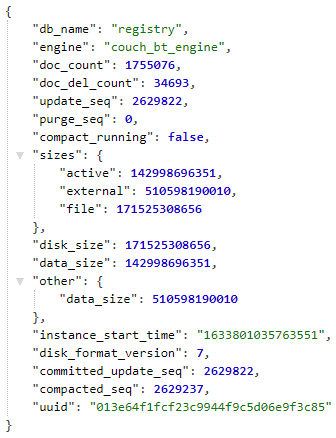
\includegraphics[scale=0.75]{images/registry_data.png}
	\caption{Az npm Registry alapadatai.}
	\label{fig:registry}
\end{figure}

A \ref{fig:registry} ábra nem reprezentálja az aktuális adatokat, mivel a közösség aktívan növeli a registryben tárolt csomagok számát és méretét, illetve bizonyos esetekben csökkenti azokat. Jól látható, hogy ekkora méretű adatbázist lokálisan nem célszerű tárolni és mivel általában a registry csomagjainak csak a töredékére van szükség, így általában felesleges is, ezért lehet hasznos a registry API, mellyel el lehet érni interneten keresztül az adatbázist.\\

\begin{flushright}
	\cite{npm-registry}
\end{flushright}

\subsection{Registry API}

A registry API \underline{Meta} végpontjai:

\begin{itemize}
	\item \texttt{GET·/}
	\item \texttt{GET·/-/all}
	\item \texttt{$\big[$GET·/-/$\big]$}
\end{itemize}

A registry API \underline{package} végpontjai:

\begin{itemize}
	\item \texttt{GET·/$\bigl\{$package$\bigr\}$}
	\item \texttt{GET·/$\bigl\{$package$\bigr\}$/$\bigl\{$version$\bigr\}$}
	\item \texttt{$\big[$GET·/-/v1/search$\big]$}
\end{itemize}

A \texttt{GET·/$\bigl\{$package$\bigr\}$} végpont válaszul egy csomag metaadat dokumentumot fog adni JSON formában. Ezeket az információkat többnyire a korábban már említett \emph{package.json} fájlból szerzi be.\\

A \texttt{$\big[$GET·/-/v1/search$\big]$} végpont a csomagok keresésében kulcsszerepet játszik és több, hasznos paramétert meg lehet adni, amely finomítja a keresést.
\textbf{Ilyen paraméterek:}

\begin{itemize}
	\item \texttt{"text"} (a keresés szövege)
	\item \texttt{"size"} (a találatok száma 20<n<250)
	\item \texttt{"from"} (honnantól kezdve adja vissza a találatokat)
	\item \texttt{"quality"} (mennyire befolyásolja a keresést a csomagok minősége [0-1])
	\item \texttt{"popularity"} (mennyire befolyásolja a keresést a csomagok népszerűsége [0-1])
	\item \texttt{"maintenance"} (mennyire befolyásolja a keresést a csomagok karbantartása  [0-1])
\end{itemize}

\pagebreak

A keresés további finomítására léteznek speciális paraméterek, ezeket azonban csak teljes szöveges lekérdezésnél lehet alkalamazni.
\textbf{Ilyen paraméterek:}

\begin{itemize}
	\item \texttt{"author:"} (Csomagok szűrése erre a szerzőre)
	\item \texttt{"maintainer:"} (Csomagok szűrése erre a fenntartóra)
	\item \texttt{"keywords:"} (Csomagok szűrése az adott kulcsszavakra, több kulcsszó esetén:)
	\begin{itemize}
		\item \texttt{','} = Logikai VAGY
		\item \texttt{'+'} = Logikai ÉS
		\item \texttt{',-'} = Kulcsszavak kihagyása
	\end{itemize}
	\item \texttt{"not:unstable"} (1.0.0-nél kisebb verziók kihagyása)
	\item \texttt{"not:insecure"} (Nem biztonságosnak megjelölt csomagok kihagyása)
	\item \texttt{"is:unstable"} (Szűrés 1.0.0-nél kisebb verziókra)
	\item \texttt{"is:insecure"} (Szűrés nem biztonságosnak megjelölt csomagokra)
	\item \texttt{"boost-exact:false"} (Ne kerüljenek fentebb az egzakt találatok (Alapértelmezett: true))
\end{itemize}

\begin{flushright}
	\cite{npm-registry-api}
\end{flushright}

\subsection{A Registry Elemek Szerkezete}

A Registry a csomagokról szöveges formában tárolja a mataadatokat. Ezeket az átláthatóság érdekében célszerű egy JSON parser kiegészítővel vizsgálni. Ekkor az alábbi formában kapható meg az adott csomagra vonatkozó információ:

\begin{figure}[h]
	\centering
	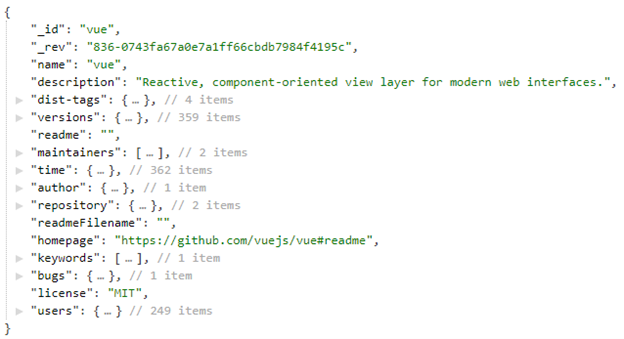
\includegraphics[scale=0.75]{images/registry_vue.png}
	\caption{Egy registry elem szerkezete. (Vue.Js)}
	\label{fig:registry-package}
\end{figure}

\pagebreak

A \ref{fig:registry-package} ábra egy \textbf{teljes verziós objektumot} ábrázol, amely a Vue.JS-ről tartalmaz metaadatokat. Itt minden \underline{felső-szintű információt} listáz az adott csomagról. \textbf{Ilyenek:}

\begin{itemize}
	\item \texttt{"\_id"} (CouchDB azonosító)
	\item \texttt{"\_rev"} (CouchDB dokumentum revíziós szám)
	\item \texttt{"name"} (A csomag neve)
	\item \texttt{"dist-tags"} (Kiadási címkék, minden csomag rendelkezik "latest" cimkével.)
	\item \texttt{"time"} (Egy olyan objektum, amely a verziókhoz köti a kiadási idejüket)
	\item \texttt{"users"} (Felhasználók akik megcsillagozták a csomagot)
	\item \texttt{"versions"} (A mindenkori verziók objektumokként listázva. Ez a projekt szempontjából kulcsfontosságú.)
\end{itemize}

A \underline{további mezőket} a a legutóbbi (latest) kiadású csomag verzió objektumhoz tartozó \emph{package.json} fájlból fogja beemelni:

\begin{itemize}
	\item \texttt{"author"} (\emph{human} objektum)
	\item \texttt{"bugs"} (Hivatkozás)
	\item \texttt{"contributors"} (\emph{human} objektumokat tartalmazó tömb)
	\item \texttt{"description"} (Csomag rövid leírása)
	\item \texttt{"homepage"} (Hivatkozás)
	\item \texttt{"keywords"} (\emph{string} kulcsszavakat tartalmazó tömb)
	\item \texttt{"license"} (A csomag licenszének \textbf{SPDX azonosítója})
	\item \texttt{"maintainers"} (Olyan \emph{human} objektumokat tartalmazó tömb, amelyeknek jogosultsága van a csomag publikálására)
	\item \texttt{"readme"} (Az első 64KB-ja a README adatot tartalmazó fájlnak)
	\item \texttt{"readmeFilename"} (A README adatot tartalmazó fájl)
	\item \texttt{"repository"} (A \emph{package.json}-ben megadott hivatkozás.)
\end{itemize}

Minden \textbf{csomag verzió objektumnak} tartalmaznia \textbf{kell} a fenti mezőket, a rövidített verzió objektumban releváns mezőit, illetve legalább a következő mezőket:
 
\begin{itemize}
	\item \texttt{"\_id"} (\emph{package@version}, például \emph{npm@1.0.0})
	\item \texttt{"\_nodeVersion"} (A publikáláshoz használt Node verziója)  
	\item \texttt{"\_npmUser"} (A csomagot publikáló felhasználó)
	\item \texttt{"\_npmVersion"} (A publikáláshoz használt npm kliens verziója)
	\item \texttt{"main"} (A csomag belépési pontja)
\end{itemize}

\textbf{A rövidített verzió objektum} a következő mezőket tartalmazhatja:

\begin{itemize}
	\item Minden esetben tartalmazza:
	\begin{itemize}
		\item \texttt{"name"} (Csomagnév)
		\item \texttt{"version"} (Csomag verzió)
		\item \texttt{"dist"} (\emph{dist} objektum)
	\end{itemize}
	\item Abban az esetben tartalmazza, ha relevánsak:
	\begin{itemize}
		\item \texttt{"deprecated"} (Elavultsági figyelmeztetések)
		\item \texttt{"dependencies"} (Szemantikus verziózással megadott függőségek)
		\item \texttt{"optionalDependencies"} (Szemantikus verziózással megadott opcionális függőségek)
		\item \texttt{"devDependencies"} (Szemantikus verziózással megadott fejlesztői függőségek)
		\item \texttt{"bundleDependencies"} (Függőségek tömbje ehhez a verzióhoz csomagolva)
		\item \texttt{"peerDependencies"} (Szemantikus verziózással megadott "peer" függőségek)
		\item \texttt{"bin"} (Ehhez a verzióhoz kötött "bin" parancsok)
		\item \texttt{"directories"} (Tömb mely olyan könytárakat tartalmaz, amelyeket tartalmaz az adott verzió)
		\item \texttt{"engines"} (Az adott verzió futtatásához szükséges Node motorok)
		\item \texttt{"\_hasShrinkwrap: true"} (Ha ismert, hogy a csomag tartalmazza, akkor "true", egyébként "false")
	\end{itemize}
\end{itemize}

\begin{flushright}
	\cite{npm-registry-item}
\end{flushright}

\begin{figure}[h]
	\centering
	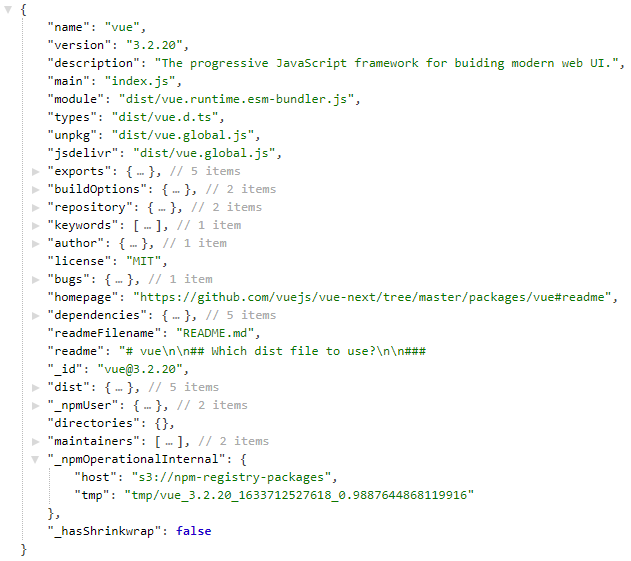
\includegraphics[scale=0.5]{images/registry_vue_version.png}
	\caption{Vue.JS@3.2.20 verzió objektum.}
	\label{fig:registry-vue-version}
\end{figure}

\pagebreak

\section{npm CLI}

Az npm CLI (Command Line Interface), azaz parancssoros felület az csomagkezelő használatának alapját adja. Segítségével telepíthetők, publikálhatók a fejlesztők által készített csomagok. Funkcionalitása széleskörű, vannak olyan csomagok, melyek csak a CLI-re támaszkodnak a felhasználóval való kommunikációhoz.

Használata egyszerű, miután települt a céleszközre, globálisan elérhető a rendszeren belül, és a definiált npm parancsokkal azonnnal igénybe vehetők a funkciói.
\begin{table}[h]
	\caption{Releváns npm CLI parancsok, a teljesség igénye nélkül:}
	\label{tab:npm-cli}
	\begin{tabularx}{\textwidth} { 
			| >{\centering\arraybackslash}X 
			| >{\centering\arraybackslash}X |}
		\hline
		\textbf{Parancs} & \textbf{Leírás} \\
		\hline
		\texttt{npm install packagename (parameters)} & Csomagok telepítése. Testvére az \texttt{npm uninstall}. Paraméterek: 
		\newline--save: mentés valamely függőségek közé
		\newline--global: globálisan telepíti a csomagot (alapértelmezett: lokális)
		\\
		\hline
		\texttt{npm exec -- <pkg>[@<version>] [args...]} & Tetszőleges parancs futtatása egy npm csomagból.
		\\
		\hline
		\texttt{npm publish [<tarball>|<folder>] [--tag <tag>] [--access <public|restricted>] [--otp otpcode] [--dry-run]]} & Csomag publikálása az npm registrybe. Testvére az \texttt{npm unpublish}.
		\\
		\hline
		\texttt{npm run-script <command> [--if-present] [--silent] [-- <args>]} & A csomagban definiált szkriptek futtatása.
		\\
		\hline
		\texttt{npm start [-- <args>]} & A csomag futtatása.
		\\
		\hline
		\texttt{npm pack [[<@scope>/]<pkg>...] [--dry-run] [--json]} & A csomagból "tarball" készítése.
		\\
		\hline
		\texttt{npm help <term> [<terms..>]} & További npm parancsok kilistázása, leírása.
		\\
		\hline
	\end{tabularx}
\end{table}

Az npm CLI alapértelmezett beállításai szerint a publikus npm Registry-t használja a csomagok adatainak lekérdezéséhez, illetve a csomagok lokális telepítéséhez. Ez azonban igény esetén megváltoztatható, tehát az npm készséggel támogatja a privát registryk használatát.

\begin{flushright}
	\cite{npm-cli}
\end{flushright}

